\documentclass[12pt, a4paper]{article}
\usepackage[utf8]{inputenc}
\usepackage{formatting}



\begin{document}

\thispagestyle{empty}

\vspace*{-1.5cm}

\noindent \textit{2024 - pt-br}

\vspace*{14pt}
{
\fontsize{32pt}{24pt}\selectfont{
    \begin{center} \bfseries{ {Guia Monitor PSoC 6}} \end{center}
	}
}
\vspace*{12pt}

\tableofcontents

\section{Montagem do Experimento}

Esta parte do guia visa mostrar o passo a passo para a montagem do experimento de Irradiação utilizando o PSoC 6.

\addcontentsline{toc}{subsection}{Pré-requisitos}
\subsection*{Pré-requisitos}

\begin{itemize}[leftmargin=1.3cm]
    \item Certifique-se que o sistema operacional não será suspenso ou desligado automaticamente nas opções de energia do computador;
    \item Obtenha o software \text{``monitor\_psoc"} para o sistema operacional escolhido através do link disponibilizado;
    \item Tenha em mãos os dois kits de desenvolvimento e os cabos USB para a conexão dos dispositivos com a interface serial do software.
\end{itemize}

\begin{figure}[H]
    \centering
    \caption{(DUT) - Kit de Desenvolvimento Infineon CY8CPROTO-063-BLE}
    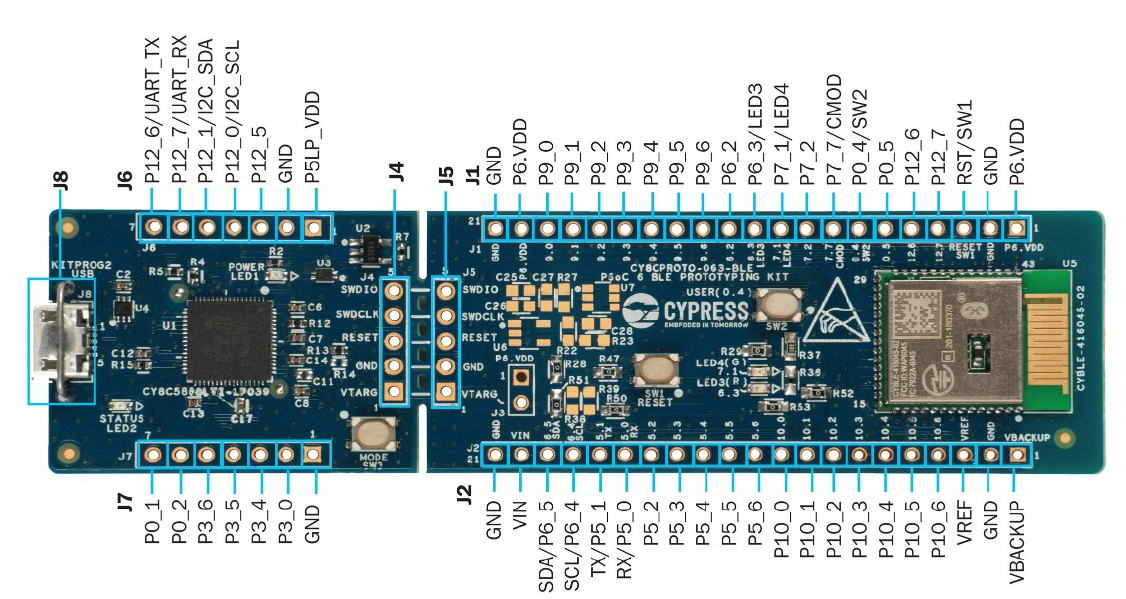
\includegraphics[width=0.5\textwidth]{../imgs/psoc63_DUT.png}

    \vspace{0.5em}
    \label{fig:psoc6}
\end{figure}

\begin{figure}[H]
    \centering
    \caption{Watchdog - Kit de Desenvolvimento Infineon CY8CPROTO-062-4343W}
    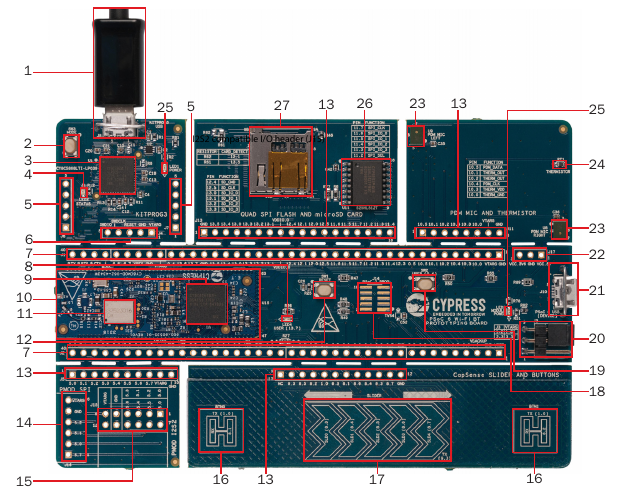
\includegraphics[width=0.5\textwidth]{../imgs/psoc62_watchdog.png}

    \vspace{0.5em}
    \label{fig:watchdog}
\end{figure}

\addcontentsline{toc}{subsection}{Etapas}
\subsection*{Etapas}

\begin{enumerate}[leftmargin=1.3cm]
    \item  Realize a conexão das placas conforme está representado no diagrama da figura abaixo:
\end{enumerate}

\begin{figure}[H]
    \centering
    \caption{Esquema de conexões para o experimento}
    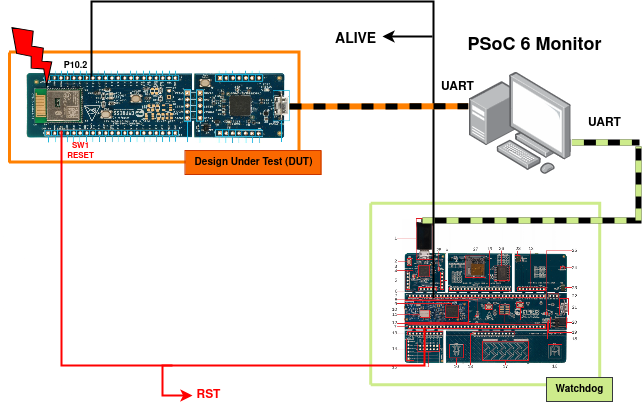
\includegraphics[width=0.8\textwidth]{../imgs/esquema_ligacoes.png}

    \vspace{0.5em}
    \label{fig:diagrama_con}
\end{figure}

\begin{enumerate}[leftmargin=1.3cm]
    \setcounter{enumi}{1}
    \item  Abra o software de monitoramento, entre em ``Start Monitoring" utilizando o teclado e escolha a porta serial que cada dispositivo está conectado.
\end{enumerate}

Para descobrir a porta serial dos dipositivos, o usuário poderá entrar em Gerenciador de Dispositivos no windows conforme a figura abaixo:

\begin{figure}[H]
    \centering
    \caption{Windows - Gerenciador de dispositivos}
    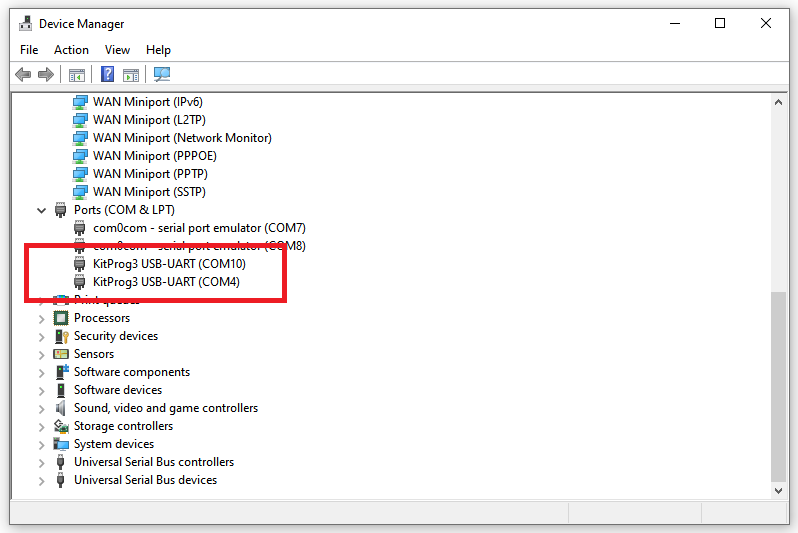
\includegraphics[width=0.7\textwidth]{../imgs/device_manager.png}

    \vspace{0.5em}
    \label{fig:device_manager}
\end{figure}

Digite a primeira porta que aparecer com o nome KitProg no campo ``PSoC 6 port" como demostrado na Figura \ref{fig:serial_windows} -- neste caso: \textbf{COM10}. Se o usuário conectar o kit errado, o software acusará ``Error connecting to port!" após de ``Attempting connection \text{...}" e então basta selecionar a outra porta serial, que seria \textbf{COM4}.

\begin{figure}[H]
    \centering
    \caption{Conectando portas seriais no Windows}
    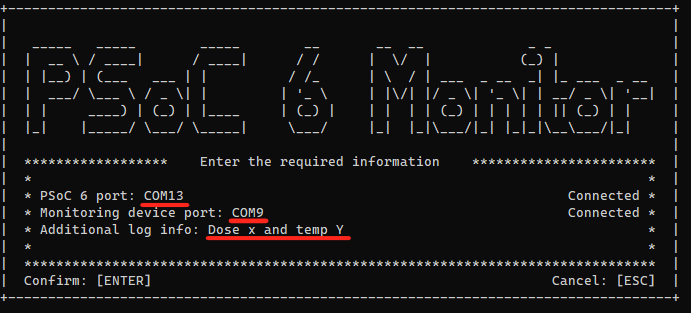
\includegraphics[width=0.8\textwidth]{../imgs/serial_windows.png}

    \vspace{0.5em}
    \label{fig:serial_windows}
\end{figure}

Se o sistema operacional for linux, as portas podem ser listadas utilizando: ``ls /dev/ttyUSB* /dev/ttyACM*".

\begin{figure}[H]
    \centering
    \caption{Conectando portas seriais no Linux}
    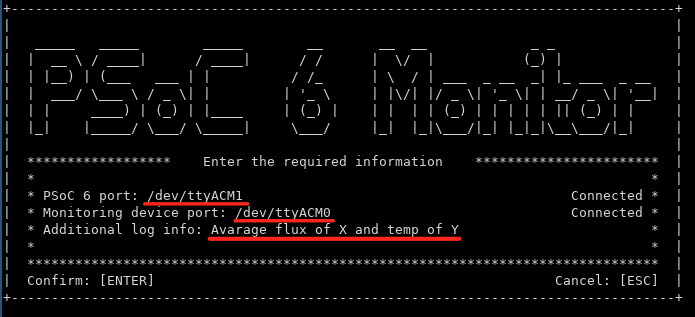
\includegraphics[width=0.8\textwidth]{../imgs/serial_linux.png}

    \vspace{0.5em}
    \label{fig:serial_linux}
\end{figure}

\begin{enumerate}[leftmargin=1.3cm]
    \setcounter{enumi}{2}
    \item Adicione informações sobre o experimento em ``Additional log info" como o fluxo de neutrons escolhido ou a temperatura do local. Essa informação será adicionada ao cabeçalho do arquivo de log da sessão iniciada.
\end{enumerate}

\textbf{Importante:} Antes de confirmar com ENTER e inicar a sessão, ligue a fonte de Neutrons; ou então, cronometre o tempo entre iniciar a sessão de monitoramento e o início da irradiação, para que possa ser descartado no futuro.

\begin{enumerate}[leftmargin=1.3cm]
    \setcounter{enumi}{3}
    \item Verifique se o experimento está sendo executado corretamente:
\end{enumerate}

Ambos os kits devem ter seus leds piscando (watchdog vermelho e DUT verde) que proporcionam uma indicação visual que o processamento está sendo realizado de acordo. Já o software de monitoramento deverá se assemelhar inicialmente ao da figura abaixo, com ambos aparelhos ``Connected", ``Error count" e ``Resets" zerados e a indicação visual de ``In progress".

\begin{figure}[H]
    \centering
    \caption{Menu de monitoramento}
    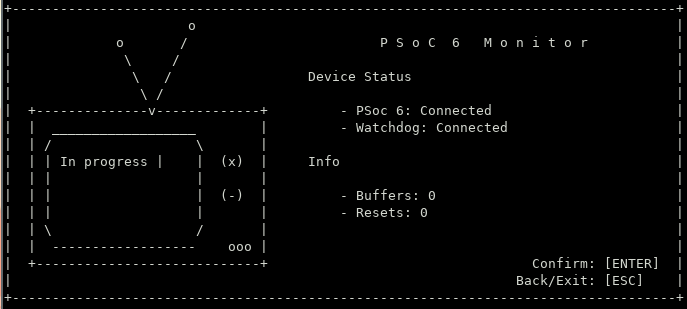
\includegraphics[width=0.8\textwidth]{../imgs/monitoring.png}

    \vspace{0.5em}
    \label{fig:monitoring_menu}
\end{figure}

\begin{itemize}[leftmargin=1.3cm]
    \item \textbf{Error count:} número de erros detectados e armazenados no arquivo de log;

    \item \textbf{Resets:} número de vezes que o PSoC 6 foi reiniciado por perda de resposta.
\end{itemize}

\begin{enumerate}[leftmargin=1.3cm]
    \setcounter{enumi}{3}

    \item Registre uma foto da montagem do experimento para ser encaminhado juntamente com os arquivos \text{.}log.

    \item Para finalizar a sessão de monitoramento corretamente, o usuário deve apertar ``ESC" e após confirmar com ``ENTER" \text{.} Feito isso, será adicionado ao final do arquivo de log um resumo da sessão com todos os dados obtidos. Os arquivos de log estarão na pasta log gerada no mesmo diretório em que foi executado o programa.
\end{enumerate}

\textbf{Importante:} A sessão de monitoramento pode ser finalizada automaticamente caso a conexão com o PSoC 6 seja completamente perdida.

Quando a conexão com o dispositivo é perdida, o programa irá fazer 7 tentativas para reviver o aparelho através do sinal de Reset. O tempo entre cada tentativa é incrementado conforme o seu número, isto é: 5, 10, 30\text{...}300s. Se nenhuma das tentativas funcionar, a sessão de monitoramento será encerrada como na figura abaixo:

\begin{figure}[H]
    \centering
    \caption{Sessão abortada}
    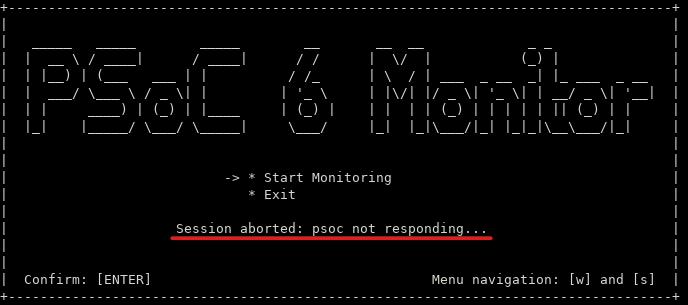
\includegraphics[width=0.8\textwidth]{../imgs/session_aborted.png}

    \vspace{0.5em}
    \label{fig:session_aborted}
\end{figure}

Visto isso, o usuário deverá desconectar os cabos USBs dos kits e realizar novamente as ligações. Caso a conexão não volte, deverá ser regravada a imagem da flash do PSoC 6 como mostrado em ``Atualizando o Firmware".

\section{Atualizando o Firmware}

Caso seja necessário regravar a imagem da flash do dispositivo, o usuário -- com o arquivo \text{.}hex em mãos -- pode utilizar o programa PSoC Programmer que é encontrado para windows pelo link: \url{https://softwaretools.infineon.com/tools/com.ifx.tb.tool.psocprogrammer}

% Image PSoc Programmer
\begin{figure}[H]
    \centering
    \caption{PSoC Programmer}
    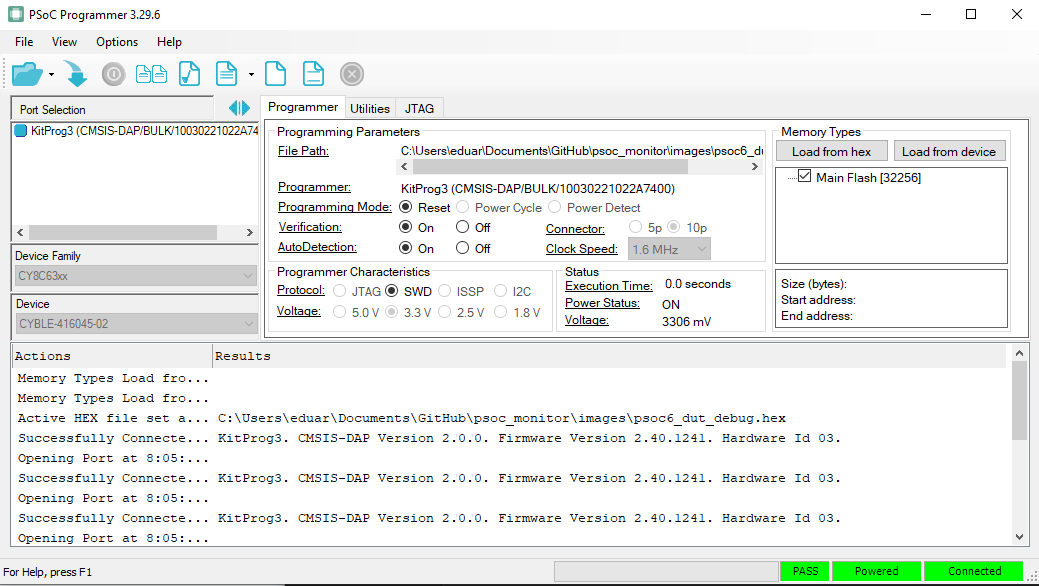
\includegraphics[width=0.8\textwidth]{../imgs/psoc_programmer.png}

    \vspace{0.5em}
    \label{fig:psoc_programmer}
\end{figure}

O passo a passo de como carregar o arquivo para o SOC é explicado no seguinte vídeo: \url{https://www.youtube.com/watch?v=aPe2A1J0OIA}

\section{Ideia do Experimento}

\begin{figure}[H]
    \centering
    \caption{Sistema desenvolvido para detecção de falhas}
    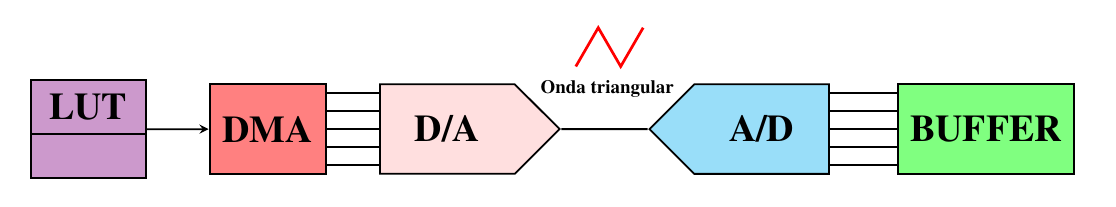
\includegraphics[width=0.8\textwidth]{../imgs/ideia_experimento.png}

    \vspace{0.5em}
    \label{fig:experiment_idea}
\end{figure}

Utilizando os conversores AD e DA do PSoC 6, é gerado um sinal de tensão triangular com frequencia de 1 kHz; ao mesmo tempo, esse sinal é lido e armazenado em um buffer de memória. A partir dos dados coletados, é verificado as características do sinal recebido e comparado com valores padrões.

\end{document}
